\documentclass[a4paper, 12pt]{article}
\usepackage[T1]{fontenc}
\usepackage[margin=0.5in]{geometry}
\usepackage{hyperref}
\usepackage{graphicx}
\usepackage{listings}
\usepackage{xcolor}

\lstset {
    language=C++,
    backgroundcolor=\color{black!5},
    basicstyle=\footnotesize,
}

\title{Dns resource record export tool}
\author{Jakub Pružinec \\
        email: j.pruzinec@gmail.com \\
        university email: xpruzi02@fit.vutbr.cz}
\date{10.11.2018}
\begin{document}
\maketitle

\abstract
{
Network monitoring is a widely practiced discipline and therefore comes in many forms. Given that one is interested in all traffic of a certain type, one is forced to capture the whole traffic and filter out the relevant data. This aproach can be implemented using the standardised library \textit{LibPcap}. In this work we focus on capturing DNS traffic and exporting resource records contained in DNS answer fields.
}

\section{Introduction}
\subsection{LibPcap}
LibPcap is an open source standardized library for live packet capturing and pcap file format parsing. Operating systems tend to abstract network layers into sockets and thus forwarding only aplication layer data to the end application. LibPcap layer is positioned between a network interface card and TCP/IP layer and provides an API for capturing data in the form it receives from the network card.

\subsection{DNS traffic}
Domain Name System, often abbreviated DNS is a distributed network protocol for (not only) translation of domain names to IP addresses.

DNS realises it's translations by a sequence of DNS requests called questions or queries and DNS responses. Queries contain domain names targeted by client applications. Responses contain DNS defined data types called resource records clustered as answers, authorities and additional groups. An example of such a resource record can be an A record used for domain name to IP address translation. These records are potentially useful for network aministrators in network analysis as they depict the intentions of client end applications. Data of different resource records varies and has to be approached individually.

\subsection{Dns-export}
Dns-export is a simple tool for extracting resource records from Dns answers and for logging them on a dedicated syslog server. Dns-export captures live traffic or parses a pcap file, parses DNS packets and logs them periodically.

\section{Usage}
\subsection{Exectution}
\textit{dns-export \textless-r pcapFile | -i interface [-t timeOut=60]\textgreater \space [-s syslogServer]}\\
The description of parameters and examples can be found in dns-export manual pages.

\subsection{Build}
Dns-export uses a \textit{make} build system. Invoking the \textit{make all} command creates an executable binary file in \textit{/build} subdirectory. If one is not present, create one with \textit{mkdir build}. Cleanup can be realized by invoking the \textit{make clean} command.

\section{Design}
\subsection{Design goals}
Dns-export is designed to be extensible, reliable, secure and easy to use. Dns-export follows the \textit{ROBUST} design philosophy and attempts to gather information even from corrupted packets.

\subsection{Support}
Dns-export supports parsing of ethernet frames, IPv4 header, IPv6 fixed and optional headers, TCP header, UDP header, DNS and DNS security extention packet parsed from live and captured communications. Dns-export extracts information from A, AAAA, CNAME, MX, NS, SOA, TXT, SPF, DNSKEY, DS, NSEC and RRSIG resource records.

\subsection{Architecture}
Input is first converted to uniform binary input using Libpcap. Binary input is processed by a parser and data is uniformly stored in a gatherer. The parsed data is then sent either once or periodically to a syslog server by a sender.
\begin{figure}[h]
    \centering
    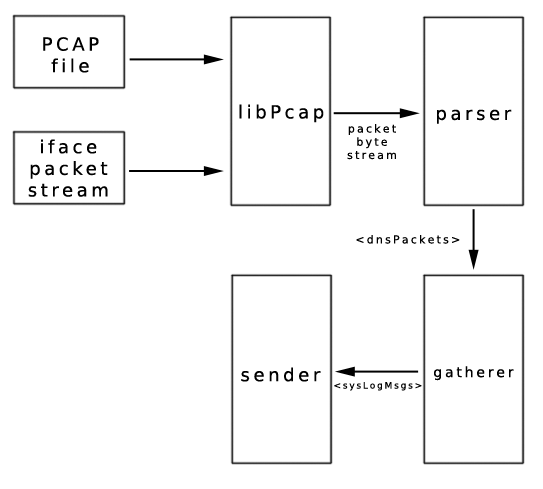
\includegraphics[width=200px]{block_scheme.png}
    \caption{Block scheme}
    \label{fig:block scheme}
\end{figure}


\newpage
\section{Implementation}
\subsection{Parser}
Link, network and transport headers except for IPv6 header are skipped by reading the data offset field and moving the position accordingly. Semantics of packet strucure fields can be found in referenced RFC literature.
\begin{lstlisting}
bool Parser::parseUdpHeader(const uint8_t *&packet, const uint8_t *packetEnd,
        struct udphdr &hdr, std::size_t &headerLen)
{
    auto packetStart = packet;
    auto udpHeader = reinterpret_cast<const struct udphdr *>(packet);

    if ((packet += sizeof(struct udphdr)) > packetEnd)
    {
        return false;
    }

    hdr.uh_sport = ntohs(udpHeader->uh_sport);
    hdr.uh_dport = ntohs(udpHeader->uh_dport);
    hdr.uh_ulen = ntohs(udpHeader->uh_ulen);
    hdr.uh_sum = ntohs(udpHeader->uh_sum);

    headerLen = packet - packetStart;
    return true;
}
\end{lstlisting}

The IPv6 fixed header is parsed first, then the parser iterates over a variable amount of optional headers, reading the offset of a next header.
\begin{lstlisting}
bool Parser::parseIPv6Header(const uint8_t *&packet, const uint8_t *packetEnd,
        uint8_t &transProt)
{
    ...
    while (nextHdr != IP_HDR_PROTOCOL_UDP && nextHdr != IP_HDR_PROTOCOL_TCP)
    {
        if (nextHdr != IP_HDR_HOPOPT && nextHdr != IP_HDR_IPV6_ROUTE &&
            nextHdr != IP_HDR_IPV6_FRAG && IP_HDR_AH)
        {
            return false;
        }
        ...
        nextHdr = packet[0];
        hdrLen = packet[1];
    }
    ...
}
\end{lstlisting}
DNS headers are fully parsed. If a parsed packet is a query, then it is discarded immediately.
\newpage
Since DNS query fields are of a variable length and preceed DNS answer fields, they must be parsed as well and are discarded afterwards. Number of queries should be declared in \textit{dqcount} DNS header field.
\begin{figure}[h]
    \centering
    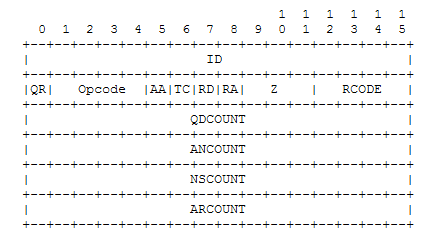
\includegraphics[width=250px]{dns_header.png}
    \caption{Dns header structure}
    \label{fig:dns header structure}
\end{figure}
\begin{figure}[h]
    \centering
    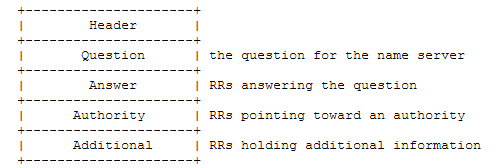
\includegraphics[width=250px]{dns_message.png}
    \caption{Dns message structure}
    \label{fig:dns message structure}
\end{figure}
\begin{lstlisting}
std::unique_ptr<DnsQuestion> Parser::parseDnsQuestion(const uint8_t *&packet,
        const uint8_t *packetStart, const uint8_t *packetEnd)
{
    std::string qname = parseDnsName(packet, packetStart, packetEnd);
    if (qname.empty())
    {
        return nullptr;
    }
    if (packet + sizeof(uint16_t) + sizeof(uint16_t) > packetEnd)
    {
        return nullptr;
    }
    ...
    return question;
}
\end{lstlisting}
\newpage
Shared fields of answer resource records are parsed uniformly and resource record data fields are parsed individually based on a declared resource record type.
\begin{lstlisting}
std::unique_ptr<DnsAnswer> Parser::parseDnsAnswer(const uint8_t *&packet,
        const uint8_t *packetStart, const uint8_t *packetEnd)
{
    ...
    uint16_t rtype = ntohs(*reinterpret_cast<const uint16_t *>(packet));
    ...
    std::unique_ptr<DnsAnswer> answer;
    switch (rtype)
    {
        case DNS_QTYPE_A:       answer = parseDnsRecordA(packet, packetEnd);
                                break;
        case DNS_QTYPE_NS:      answer = parseDnsRecordNS(packet,
                                                packetStart, packetEnd);
                                break;
        ...
        default:                answer = nullptr;
                                break;
    }
    ...
    return answer;
}
\end{lstlisting}
Some of resource records data share fragments of the same type. These fragments are parsed uniformly. 
The identical fragments are:
\begin{itemize}
\item Domain name\\
Domain name as described by RFC is parsed recursively with a limited maximum depth due to security concerns.
\end{itemize}
\begin{lstlisting}
::string Parser::parseDnsName(const uint8_t *&packet,
        const uint8_t *packetStart, const uint8_t *packetEnd, uint8_t n)
{
    ...
    uint8_t nChars = 0;
    for (; packet != packetEnd && *packet; packet++)
    {
        if (nChars == 0)
        {
            nChars = *packet;
            if (DNS_IS_POINTER(nChars))
            {
                auto pointer = reinterpret_cast<const uint16_t *>(packet);
                ...
                auto offset = DNS_OFFSET_FROM_POINTER(ntohs(*pointer));
                ...
                auto res = parseDnsName(rest, packetStart, packetEnd, n - 1);
                ...
                return domainName + res;
            }
            ...
            continue;
        }
        domainName.push_back(static_cast<char>(*packet));
        nChars--;
    }
    ...
    return domainName;
}
\end{lstlisting}
\begin{itemize}
\item Binary data\\
Binary, or context dependent data is represented in base64 notation. Since most of the data length is context dependent, it's calculated from \textit{rdlength} DNS answer field.
\end{itemize}
\subsection{Gatherer}
Data is gathered as a data string mapped to a counter of occurences.
\begin{lstlisting}
void DnsCapture::addStatistic(const std::string &recordData)
{
    auto it = statistics.find(recordData);

    if (it == statistics.end())
    {
        statistics.insert(std::make_pair(recordData, 1));
    }

    else
    {
        it->second++;
    }
}
\end{lstlisting}
\subsection{Sender}
    The sending thread is periodically woken up. It uses a UDP transport protocol mechanism with a fire and forget approach. Since the gathered statistics is a resource shared among the gathering and sending threads a mutex is used in order to prevent race conditions. The gatherer buffers statistics while the mutex is locked and stores them afterwards.
\begin{lstlisting}
bool DnsCapture::sendStatisticsToSyslogServer(void) const
{
    ...
    for (const auto &stat : statistics)
    {
        auto m = toSyslogMsg(stat.first, stat.second);
        if (send(syslogServerSock, m.c_str(), m.size(), 0) < 0)
        {
            noError = false;
        }
    }
    return noError;
}
\end{lstlisting}
\begin{lstlisting}
void sender(void)
{
    ...
    while (!global::quit)
    {
        ...
        sleep(toSleep);
        while (!global::dnsCapture->lockStatisticsMutex())
        {
            sleep(1);
            ...
        }
        global::dnsCapture->sendStatisticsToSyslogServer();
        global::dnsCapture->unlockStatisticsMutex();
    }
}
\end{lstlisting}
\newpage
\subsection{Debugging}
The dns-export source code offers a variety of dumping methods usable for further development.
\begin{lstlisting}
void Parser::dumpDnsHeader(const struct dnshdr &hdr)
{
    std::cerr << "Dns_id:\t\t\t" << hdr.id << std::endl;
    std::cerr << "Dns_qr:\t\t\t" << hdr.qr << std::endl;
    std::cerr << "Dns_opcode:\t\t" << hdr.opcode << std::endl;
    ...
}
\end{lstlisting}
\section{Restrictions}
The dns-export tool does not take network layer data fragmentation and transport layer segmentation into consideration.
\section{Conclusion and examples}
The dns-export tool is handy in dns traffic monitoring and due to it's defensive implementation approach
is suitable for daemonization to run as a monitoring service.
\subsection{Examples}
\begin{lstlisting}
./dns-export -r /Data/tmp/test/dns_aaaa.pcapng

<134>1 2018-11-17T14:05:21.003Z dankpad dns-export 20230 - - -
    [star-mini.c10r.facebook.com A 31.13.84.36] 1
<134>1 2018-11-17T14:05:21.003Z dankpad dns-export 20230 - - -
    [star-mini.c10r.facebook.com AAAA
    2a03:2880:f107:0083:face:b00c:0000:25de] 1
<134>1 2018-11-17T14:05:21.003Z dankpad dns-export 20230 - - -
    [www.facebook.com CNAME star-mini.c10r.facebook.com] 2
\end{lstlisting}
\section{Literature and sources}
Examples for ISA course by Petr Matousek\\
\url{https://stackoverflow.com/questions/1491660/pcap-struct-pcap-pkthdr-len-vs-caplen}\\
\url{https://www2.cs.duke.edu/courses/fall16/compsci356/DNS/DNS-primer.pdf}\\
\url{https://0x00sec.org/t/dns-header-for-c/618}\\
\url{https://www.ietf.org/rfc/rfc4033.txt DNSSEC}\\
\url{https://www.ietf.org/rfc/rfc4034.txt DNSSEC RR FORMATS}\\
\url{https://tools.ietf.org/html/rfc7208 SPF}\\

\end{document}